	\documentclass[final]{beamer}

% Load beamerposter for vertical A0 sizing
\usepackage[size=a0,orientation=portrait,scale=1.4]{beamerposter}
\usetheme{IITiSPoster} % Loads your .sty file

% Metadata
\title{Quantum-inspired dynamical models on quantum and classical annealers}


\author{
	Philipp Hanussek$^{1,2}$,
	Jakub Paw\l{o}wski$^{3,4}$,
	Zakaria Mzaouali$^{5,6}$,
	Bart\l{o}miej Gardas$^{1}$
}

\institute{
	$^1$ Polish Academy of Sciences, Gliwice, Poland \\
	$^2$ Sorbonne Université, Paris, France \\
	$^3$ Wrocław University of Science and Technology, Wrocław, Poland \\
	$^4$ Quantumz.io, Warsaw, Poland \\
	$^5$ Jülich Supercomputing Centre, Germany \\
	$^6$ Universität Tübingen, Germany
}
\date{May 2026}
\begin{document}
\begin{frame}[t]
	\begin{columns}[t]

		% LEFT COLUMN
		\begin{column}{.48\paperwidth}

			\begin{block}{Introduction}
				\textbf{We propose a practical, physics-inspired benchmarking suite to challenge both quantum and classical computers by mapping real-time quantum dynamics to a common optimization format.}
				\newline

				\centering
				\begin{minipage}{0.48\linewidth}
					\centering
					(a)
					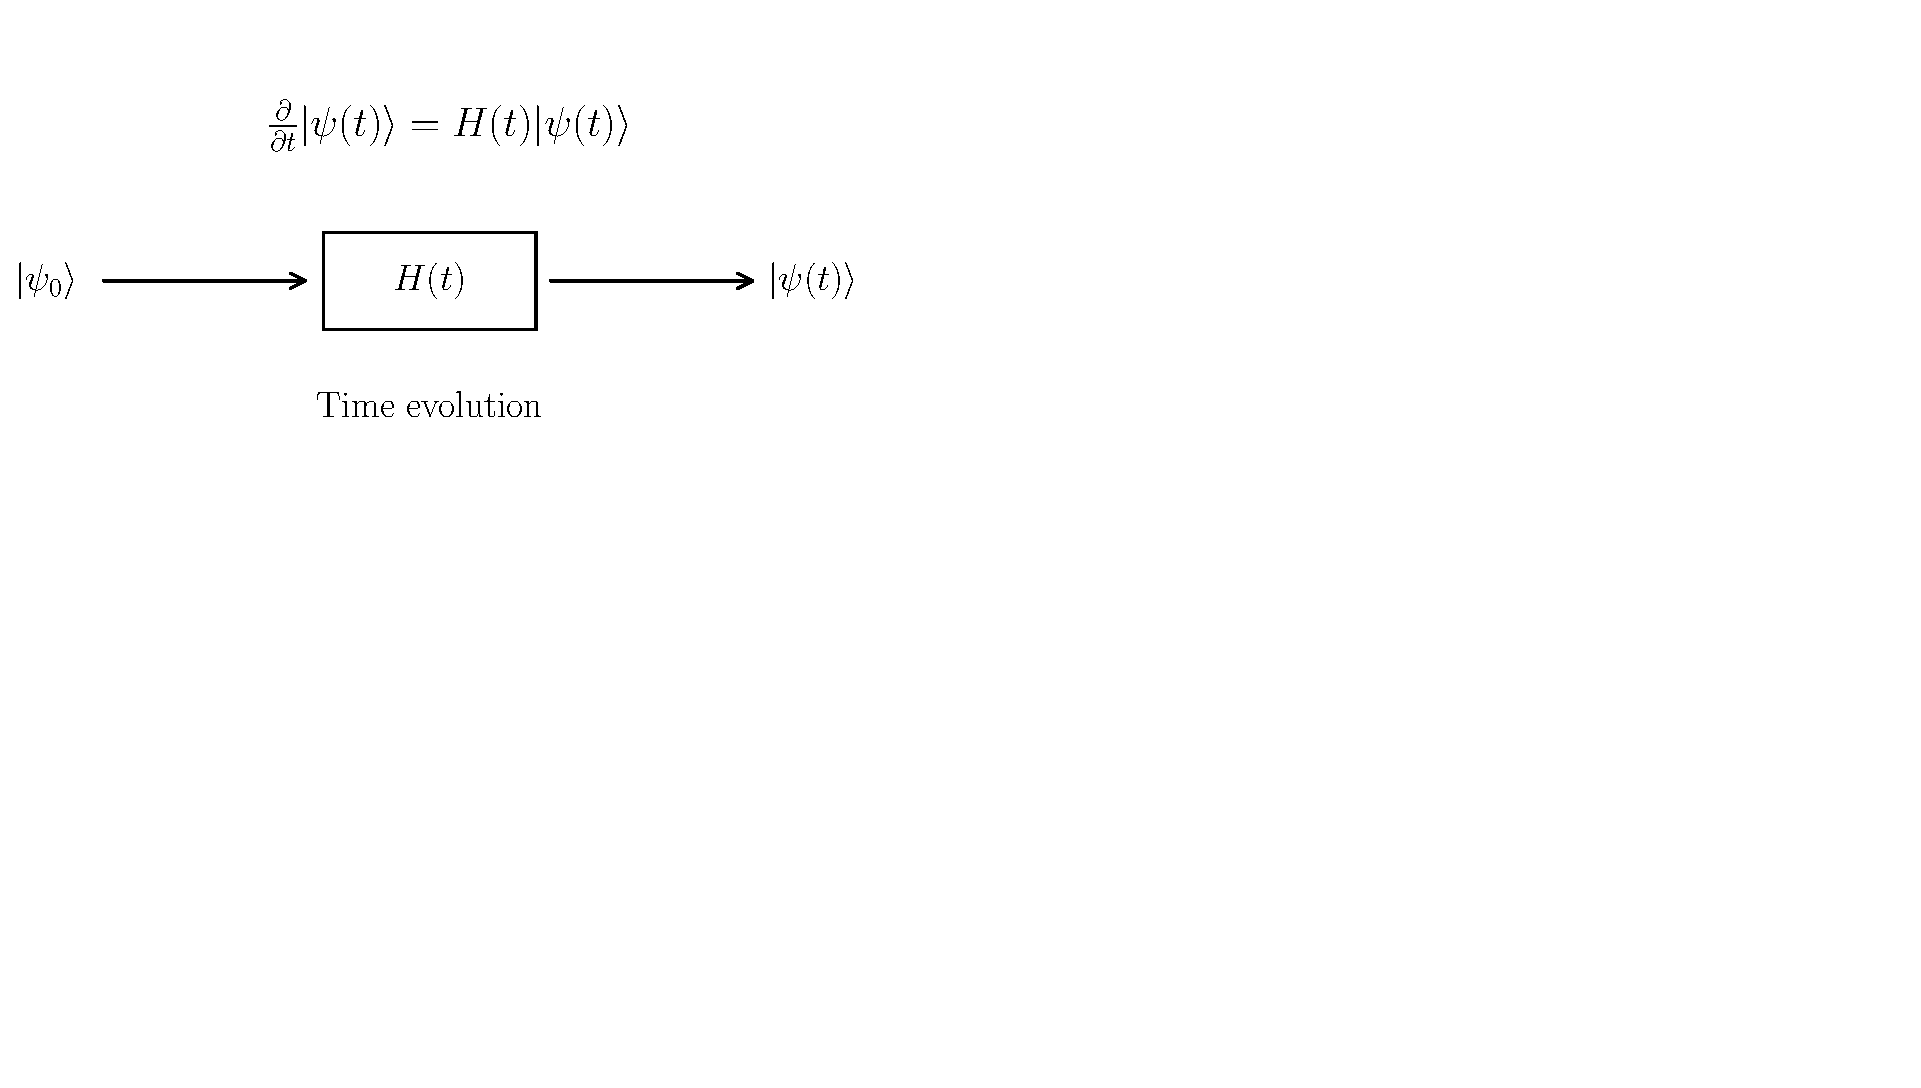
\includegraphics[width=\linewidth]{figures/1_time_eval.pdf}
				\end{minipage}
				\hfill
				% Row 1
				\begin{minipage}{0.48\linewidth}
					\centering
					(b)
					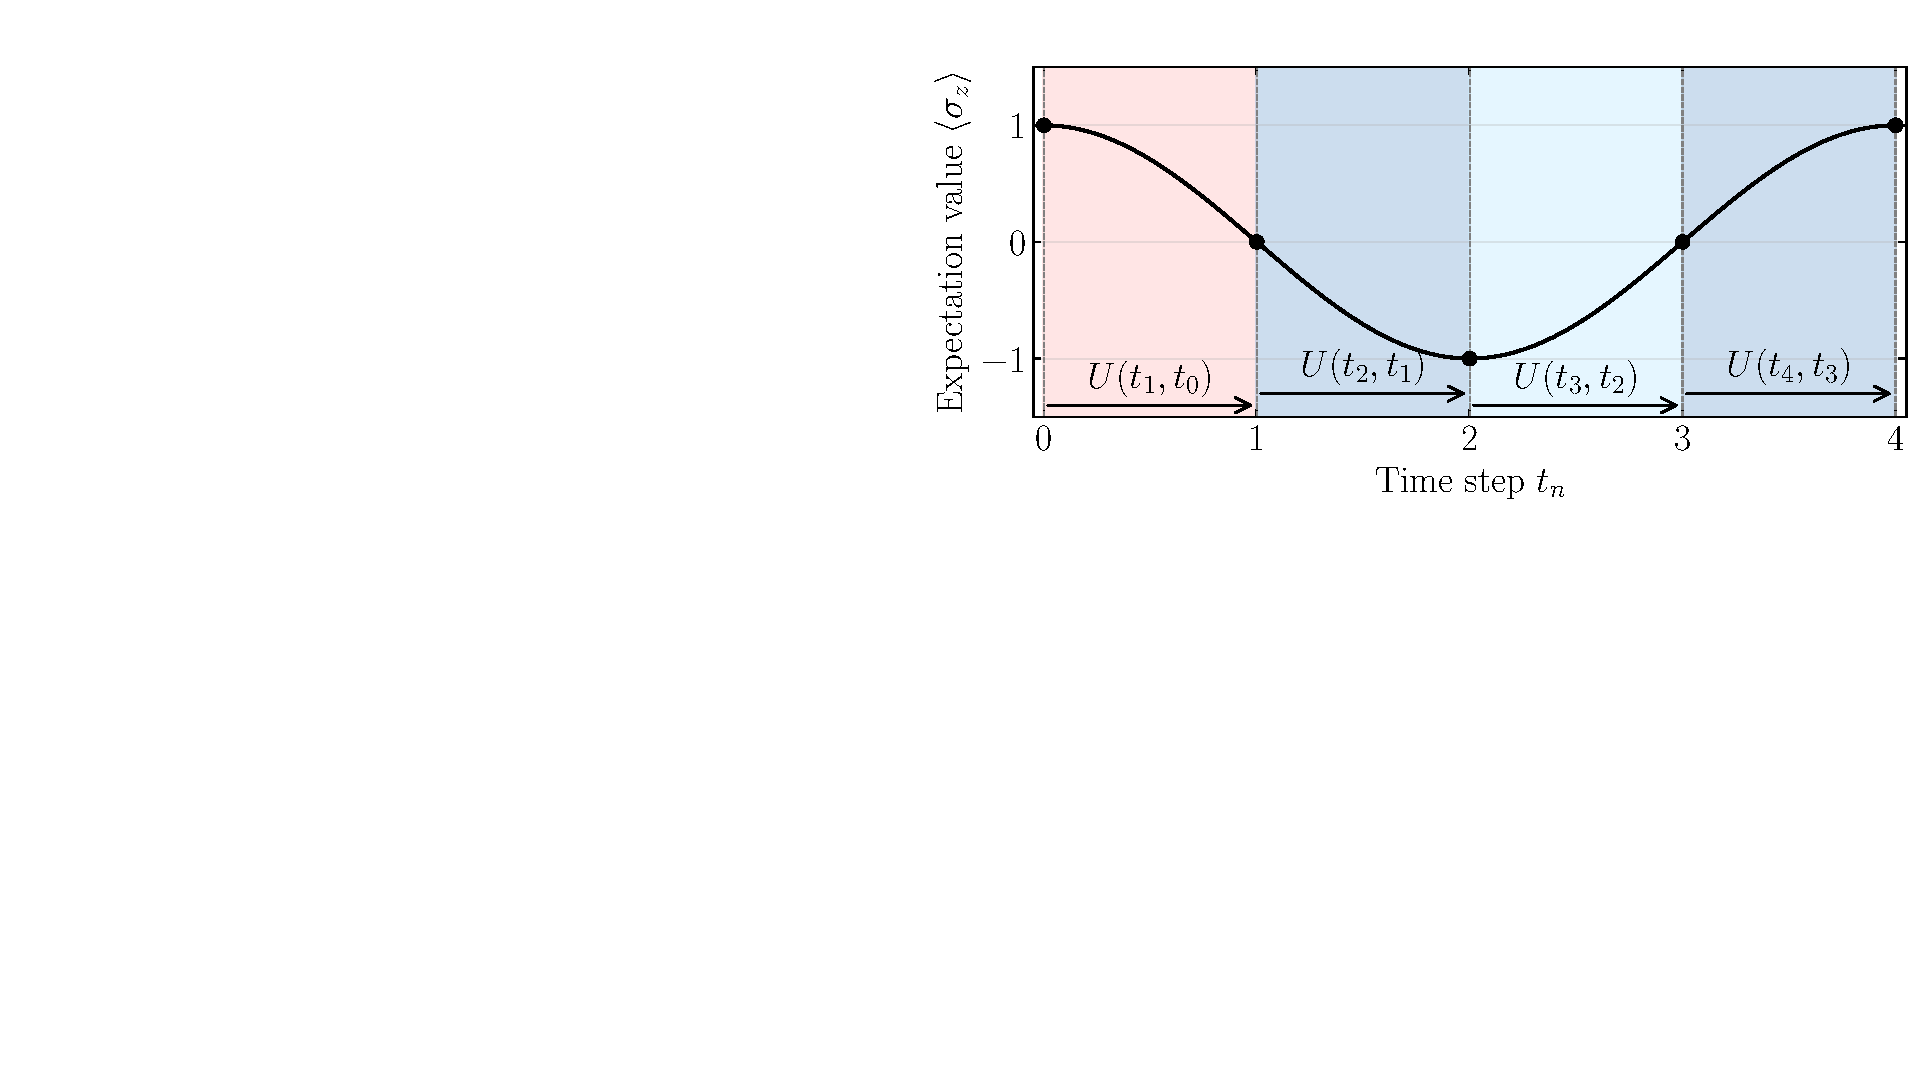
\includegraphics[width=\linewidth]{figures/2_time_evolution.pdf}
				\end{minipage}

				\vspace{1em}

				% Row 2
				\begin{minipage}{0.48\linewidth}
					\centering
					(c)
					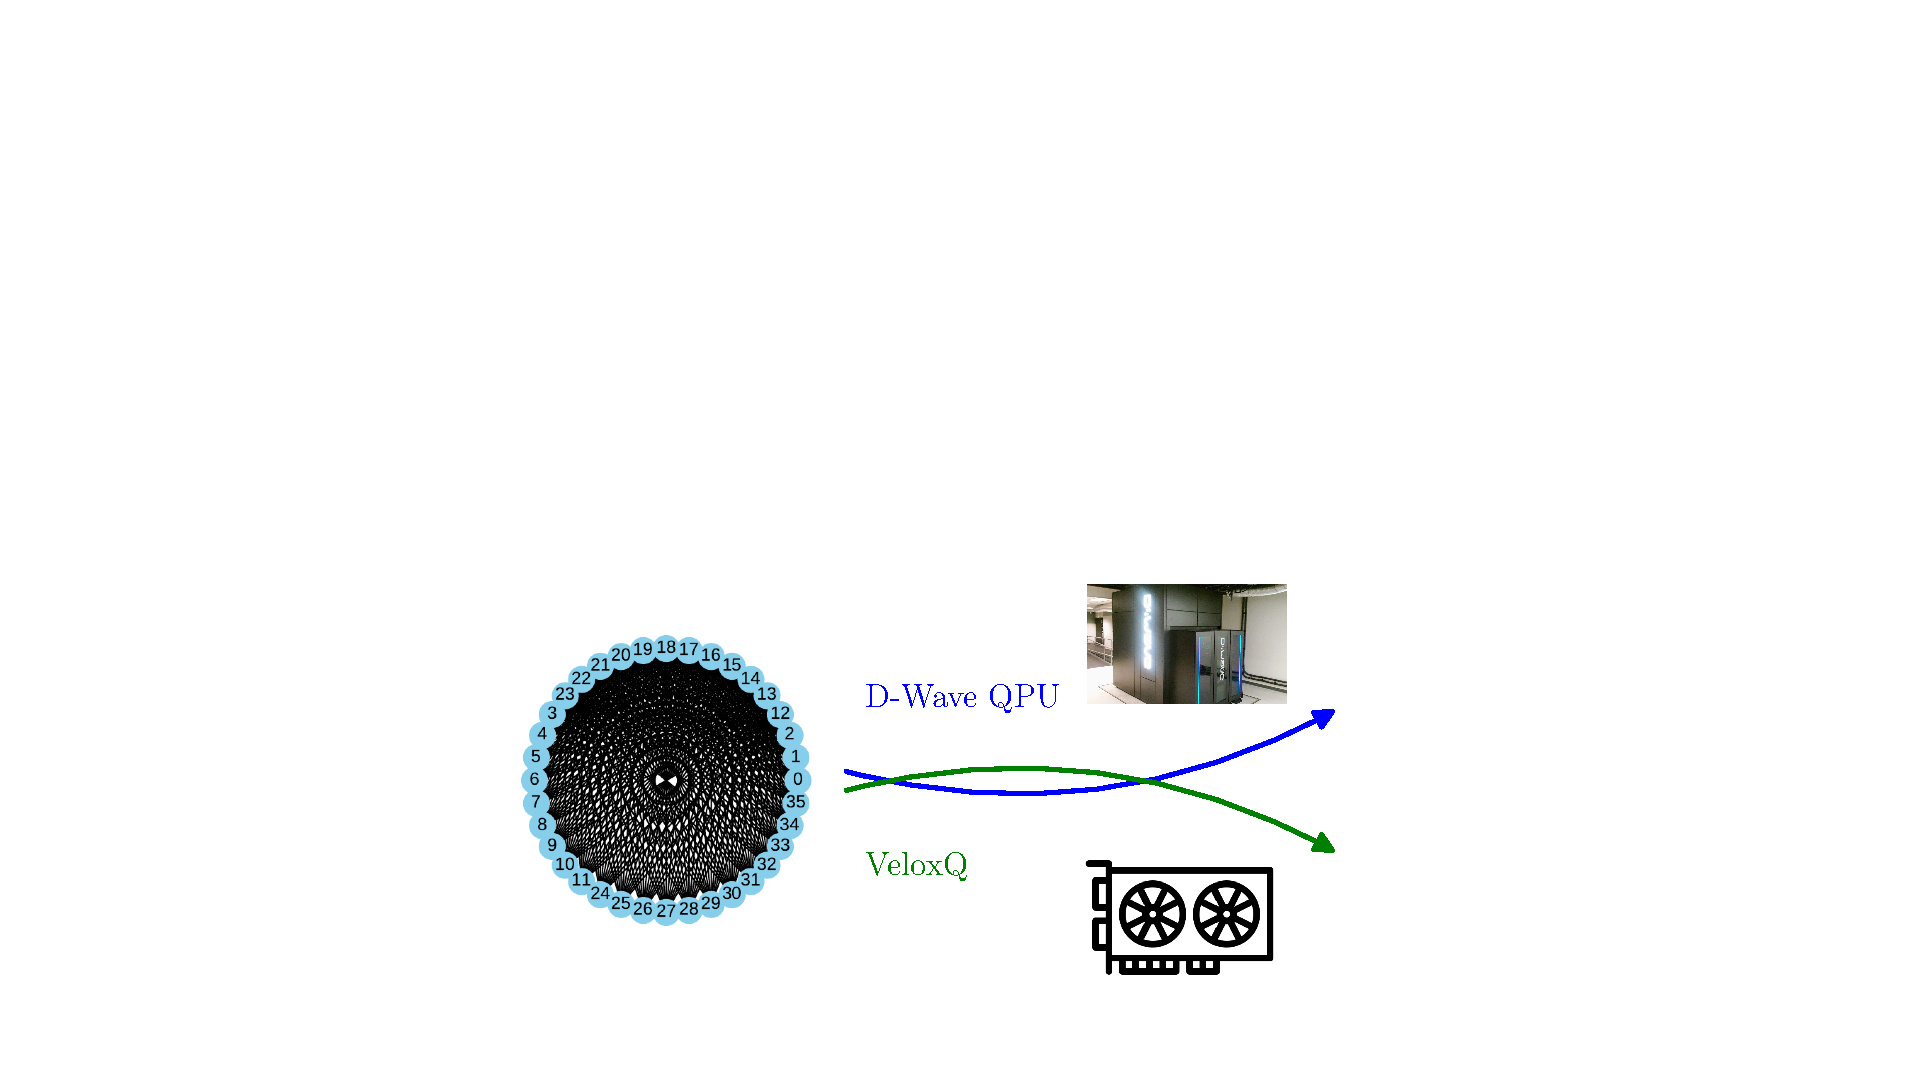
\includegraphics[width=\linewidth]{figures/4_dyn.pdf}
				\end{minipage}
				\hfill
				\begin{minipage}{0.48\linewidth}
					\centering
					(d)
					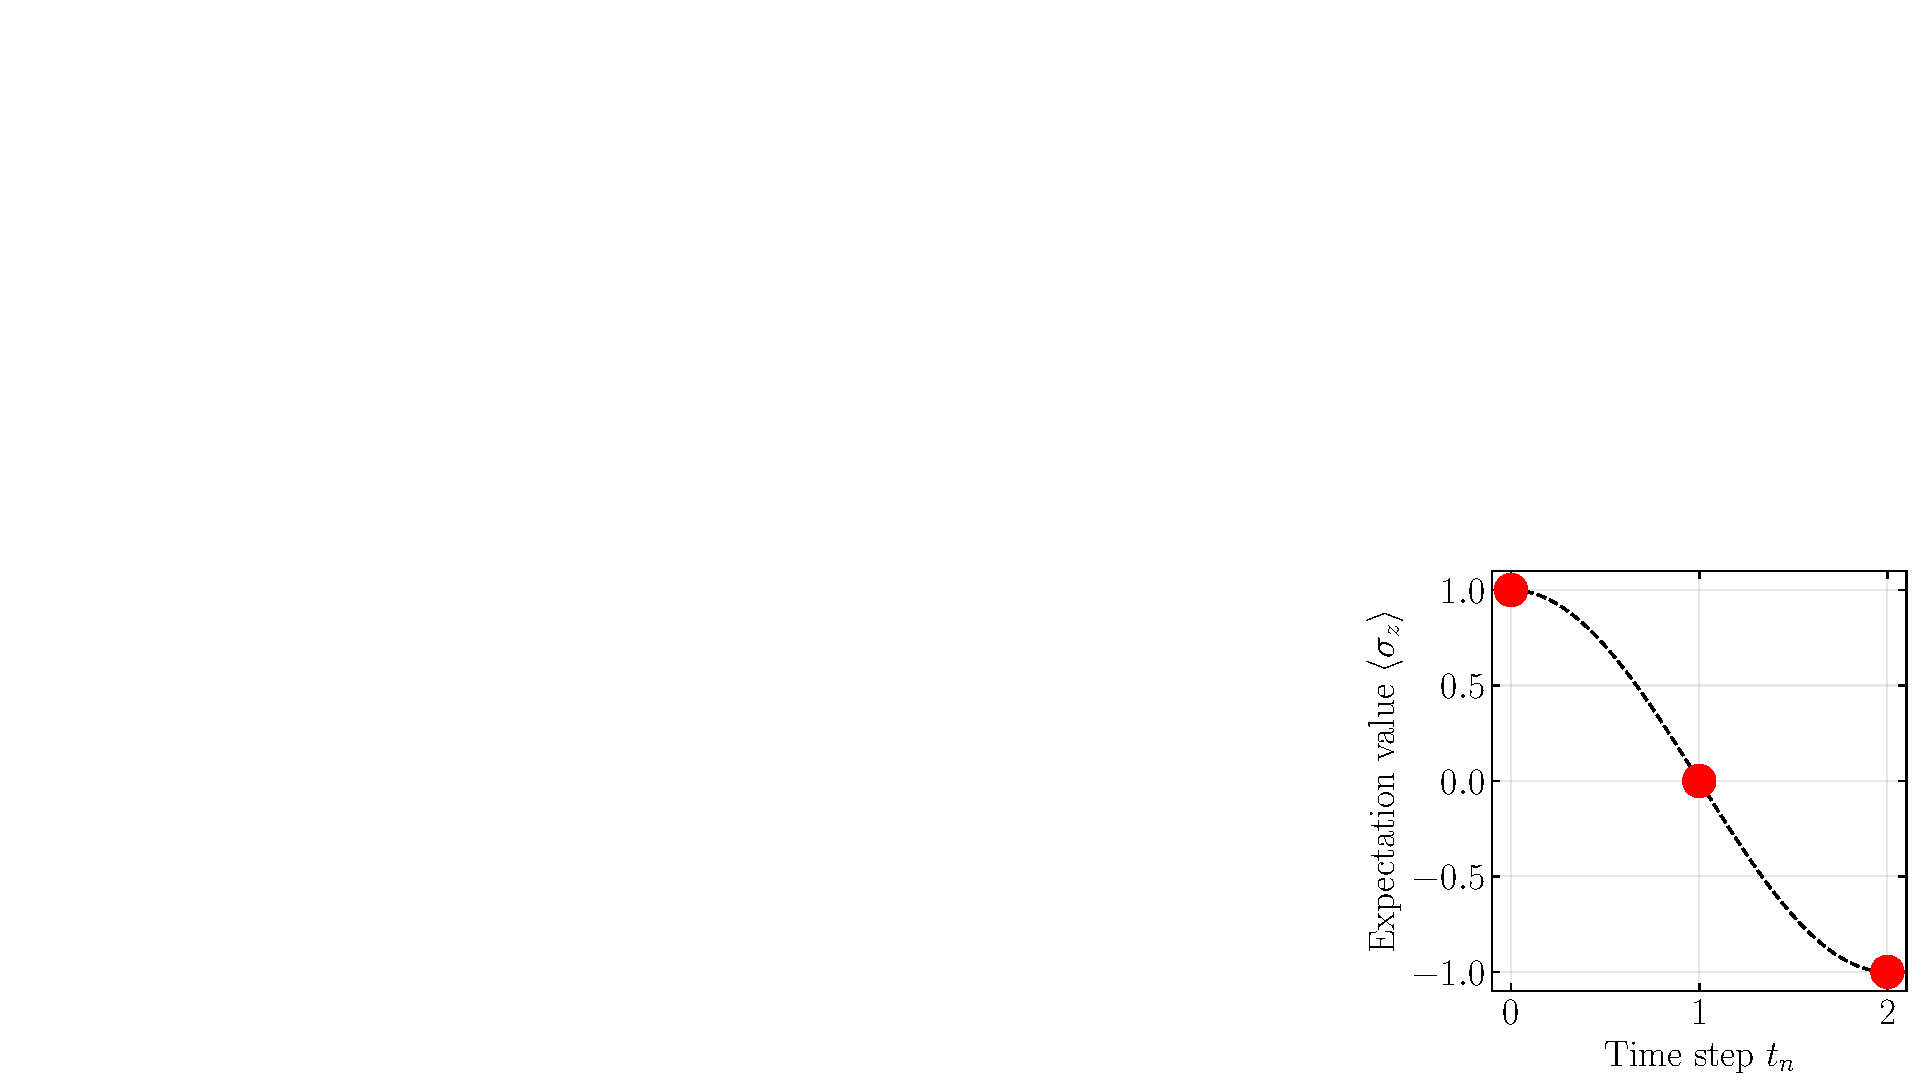
\includegraphics[width=\linewidth]{figures/5_sys.pdf}
				\end{minipage}

			\end{block}

			\begin{block}{Methods}

				\textbf{Quantum Annealing}

				\begin{itemize}
					\item Driver Hamiltonian:
					      \begin{equation*}
						      \ket{+}^{\otimes N} = \frac{1}{\sqrt{2^N}} \sum_{x \in \{0,1\}^N} \ket{x}
					      \end{equation*}
					      where $N$ is the number of qubits.
				\end{itemize}

				\vspace{-0.5em}

				\begin{columns}
					\column{0.6\linewidth}
					\begin{itemize}
						\item Problem Hamiltonian:
						      \begin{equation*}
							      H_P = \sum_{i=1}^{N} h_i \widehat\sigma_z^{(i)} + \sum_{i<j} J_{ij} \widehat \sigma_z^{(i)} \widehat \sigma_z^{(j)}.
						      \end{equation*}

						\item System evolution:
						      \begin{equation*}
							      H_\text{Ising}=\frac{A(s)}{2}H_D+\frac{B(s)}{2}H_P.
						      \end{equation*}
					\end{itemize}

					\column{0.4\linewidth}
					\centering
					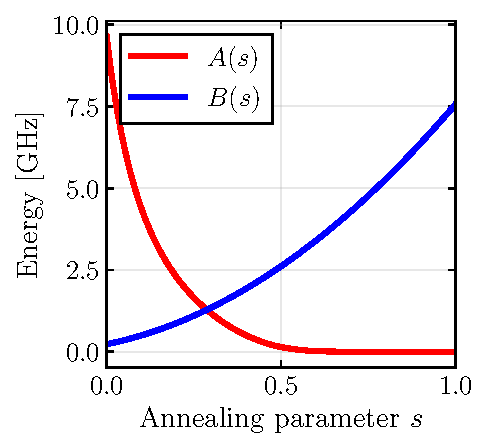
\includegraphics[width=\linewidth]{figures/anneal_schedule_plot.pdf}
				\end{columns}

				\vspace{0.5em}

				\textbf{VeloxQ}

				VeloxQ is a fast and efficient, physics-inspired solver based on the theory of dynamical systems, designed for solving QUBO problems.

			\end{block}
		\end{column}


		% RIGHT COLUMN
		\begin{column}{.48\paperwidth}
			\begin{block}{Problem Description}
				\begin{itemize}
					\item Quantum State Evolution

					      \begin{equation*}
						      \ket{\Psi} = \sum_{n=0}^{N-1} \ket{t_n} \otimes \ket{\psi(t_n)}.
					      \end{equation*}

					\item Annihilated by Hermitian clock operator

					      \begin{minipage}{0.58\linewidth}
						      \begin{equation*}
							      \begin{aligned}
								      \mathcal{C} = \sum_{n=0}^{N-2} \Big(
								       & \ket{t_{n+1}}\bra{t_{n+1}} \otimes I               \\
								       & - \ket{t_{n+1}}\bra{t_n} \otimes U_n + \text{h.c.}
								      \Big)
							      \end{aligned}
						      \end{equation*}
					      \end{minipage}
					      \hfill
					      \begin{minipage}{0.38\linewidth}
						      \centering
						      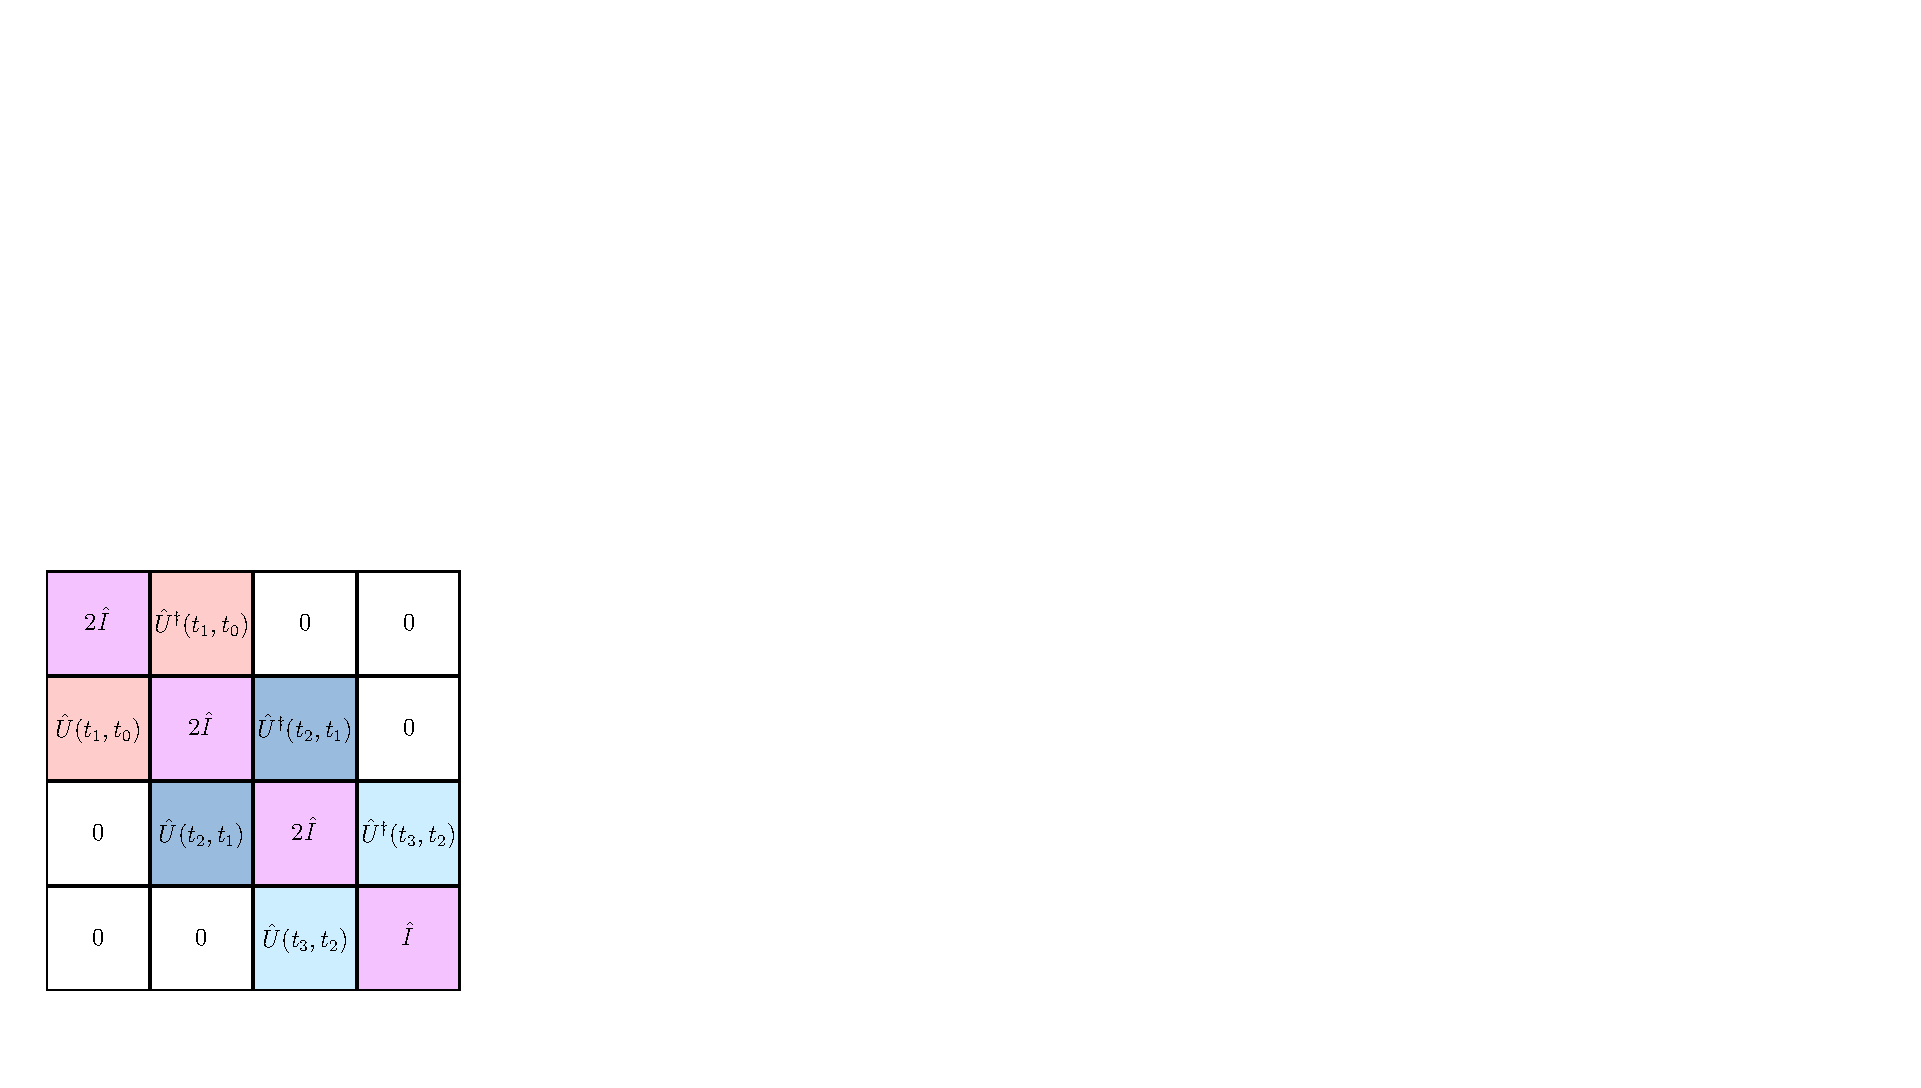
\includegraphics[width=\linewidth]{figures/3_clock.pdf}
						      Clock Hamiltonian $C$
					      \end{minipage}
					      \hfill
					\item Finally minimize
					      \begin{equation*}
						      f(\mathbf{x}) = \frac{1}{2} \bra{\mathbf{x}} \mathcal{A} \ket{\mathbf{x}} - \bra{\mathbf{x}} \phi \rangle\text{ , with } \mathcal{A} := \mathcal{C} + \ket{t_0}\bra{t_0} \otimes I
					      \end{equation*}
				\end{itemize}
				
				\textbf{Solving process}
				\begin{figure}
					\centering
					\subfloat[Example embedding on QPU\label{h1_pegasus}]{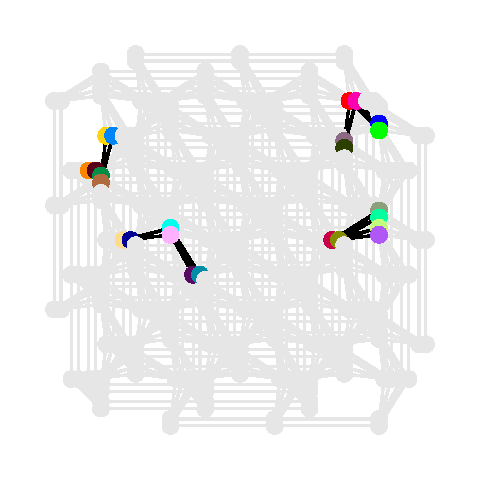
\includegraphics[width=0.3\linewidth]{figures/emb_system_2_pegasus.pdf}}%
					\subfloat[Success rates for systems $\widehat H_2$ $\widehat H_3$ \label{proba_h2h3}]{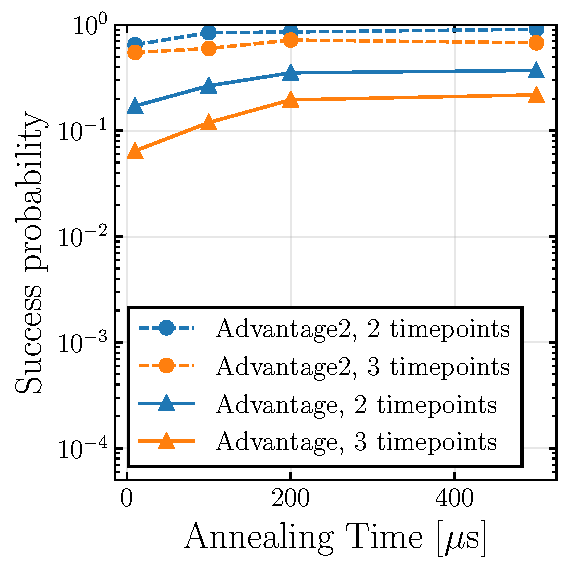
\includegraphics[width=0.3\linewidth]{figures/system_1_ta.pdf}}%
					\subfloat[Expectation value $\langle\sigma_{z}\rangle$\label{sigmaz_1}]{
\includegraphics[width=0.3\linewidth]{figures/dynamics_system_1_list.pdf}}
				\end{figure}


			\end{block}


			\begin{block}{Results}
				\begin{enumerate}
					\item Data Collection.
					\item Signal Processing.
					\item Result Verification.
				\end{enumerate}
			\end{block}

			\begin{block}{Conclusion}
				The footer automatically includes the website and institution name as requested in your footline command.
			\end{block}


		\end{column}

	\end{columns}
\end{frame}
\end{document}
